\documentclass[final]{article}

\usepackage{APS360}
\usepackage[utf8]{inputenc}
\usepackage[T1]{fontenc}
\usepackage{hyperref}
\usepackage{url}
\usepackage{booktabs}
\usepackage{amsfonts}
\usepackage{nicefrac}
\usepackage{microtype}
\usepackage{xcolor}
\usepackage{graphicx}
\usepackage{tikz}
\usetikzlibrary{positioning, arrows.meta, fit, backgrounds}
\renewcommand{\arraystretch}{0.88}
\setlength{\abovecaptionskip}{3pt}
\setlength{\belowcaptionskip}{0pt}
\setlength{\textfloatsep}{6pt plus 2pt minus 2pt}
\setlength{\floatsep}{4pt plus 2pt minus 2pt}
\setlength{\intextsep}{4pt plus 2pt minus 2pt}
\setlength{\parskip}{3pt plus 1pt minus 1pt}

% Every number cited in final_report.tex prose is defined here, sourced from
% a specific logged file, so the report can never drift from the underlying
% JSON. FINAL (not provisional) as of the 3-seed final retrain + blind
% ablation in outputs/results_final/. Only the new-data (Tier 2) macros
% remain TBD, pending the user's own collected photos -- see
% /home/olipet24/.claude/plans/vectorized-sprouting-shore.md Phase F.
%
% Headline checkpoints for qualitative work / single-run figures: seed 360.
% Test acc/loss reported in prose and Table 1 are 3-seed means (seeds
% 360/361/362); per-type breakdown and confidence stats are from the
% seed-360 checkpoint specifically (outputs/results_final/*_seed360_test_analysis.json).

% -- baseline (source: outputs/results_final/baseline_seed{360,361,362}_metrics.json) --
\newcommand{\baselineParams}{2{,}574{,}696}
\newcommand{\baselineSize}{9.84MB}
\newcommand{\baselineTestAcc}{47.43\%}
\newcommand{\baselineTestAccStd}{0.44\%}
\newcommand{\baselineTestLoss}{1.60}
\newcommand{\baselineAccYN}{58.19\%}
\newcommand{\baselineAccOther}{43.23\%}
\newcommand{\baselineAccNum}{29.84\%}
\newcommand{\baselineTunedDropout}{0.1 (default)}
\newcommand{\baselineTunedWeightDecay}{0.01 (default)}
\newcommand{\baselineTunedLR}{$1{\times}10^{-3}$}

% -- primary (source: outputs/results_final/primary_seed{360,361,362}_metrics.json) --
\newcommand{\primaryParams}{3{,}071{,}096}
\newcommand{\primarySize}{11.76MB}
\newcommand{\primaryTotalSize}{13.63MB}
\newcommand{\primaryTestAcc}{45.76\%}
\newcommand{\primaryTestAccStd}{0.31\%}
\newcommand{\primaryTestLoss}{1.64}
\newcommand{\primaryAccYN}{58.00\%}
\newcommand{\primaryAccOther}{39.45\%}
\newcommand{\primaryAccNum}{28.95\%}
\newcommand{\primaryTunedDropout}{0.2}
\newcommand{\primaryTunedWeightDecay}{0.01 (default)}
\newcommand{\primaryTunedK}{16}
\newcommand{\primaryTunedPool}{last (default; \texttt{last\_real} tested, did not help)}

% -- floors / ablations (source: outputs/results_final/primary_blind_metrics.json, test split) --
\newcommand{\majorityFloor}{21.84\%}
\newcommand{\blindFloor}{37.94\%}

% -- confidence calibration (source: *_seed360_test_analysis.json) --
\newcommand{\baselineConfCorrect}{0.63}
\newcommand{\baselineConfIncorrect}{0.48}
\newcommand{\primaryConfCorrect}{0.61}
\newcommand{\primaryConfIncorrect}{0.45}

% -- efficiency (source: outputs/results_final/efficiency.json, batch=32, Tq=16) --
\newcommand{\primaryLatencyMs}{3.4ms}
\newcommand{\baselineLatencyMs}{1.3ms}

% -- new data (source: outputs/results_new_data/new_data_summary.json; BLOCKED on user photos) --
\newcommand{\newDataN}{TBD}
\newcommand{\newDataBaselineAcc}{TBD}
\newcommand{\newDataBaselineCI}{TBD}
\newcommand{\newDataPrimaryAcc}{TBD}
\newcommand{\newDataPrimaryCI}{TBD}
\newcommand{\newDataMajorityFloor}{TBD}

% -- misc --
\newcommand{\testSetSize}{186{,}489}
\newcommand{\testSetYN}{80{,}539}
\newcommand{\testSetOther}{80{,}930}
\newcommand{\testSetNum}{25{,}020}
\newcommand{\trainPoolSize}{368{,}751}
\newcommand{\vocabCoverage}{87.47\%}


\title{Mini-VLM: A Pure RWKV Vision-Language Model for Efficient Visual Question Answering}

\author{%
  Oliver Petrovic \\
  1008923042, oliver.petrovic@mail.utoronto.ca\\
  \url{https://github.com/Olipet24/mini-vlm}\\
}

\begin{document}

\maketitle

\vspace{-0.5in}

\section*{Introduction}

Modern Vision-Language Models (VLMs) require billions of parameters and huge GPU resources,
making them impossible to run on everyday or mobile hardware. Mini-VLM is a compact VLM for
Visual Question Answering (VQA) constrained to a strict \textbf{100MB storage budget}, targeting
edge deployment: given a $224\times224$ image and a free-form text question, the model outputs one
of the 1000 most common VQA answers (Figure~\ref{fig:pipeline}). Mapping raw pixels and free-form
text jointly onto a correct answer requires learned, non-linear visual and linguistic
representations that hand-coded rules cannot approximate (Goyal et al., 2017), which is why deep
learning is appropriate here. Rather than shrinking a Transformer-based VLM post hoc, our core
contribution is a \emph{unified RWKV pipeline}: an RWKV spatial bridge and language core replace
attention everywhere, giving linear-time (not quadratic) cost in the combined visual+text sequence
length (Peng et al., 2023), instead of the linear-projector-into-attention approach used by
connectors such as LLaVA (Liu et al., 2023). We compare this directly against a control baseline
that keeps the same frozen encoder but restores standard self-attention, and evaluate both on the
full VQA v2.0 pool, a held-out test split, and newly collected photographs never used in tuning.

\begin{figure}[!htbp]
  \centering
  \resizebox{\linewidth}{!}{%
  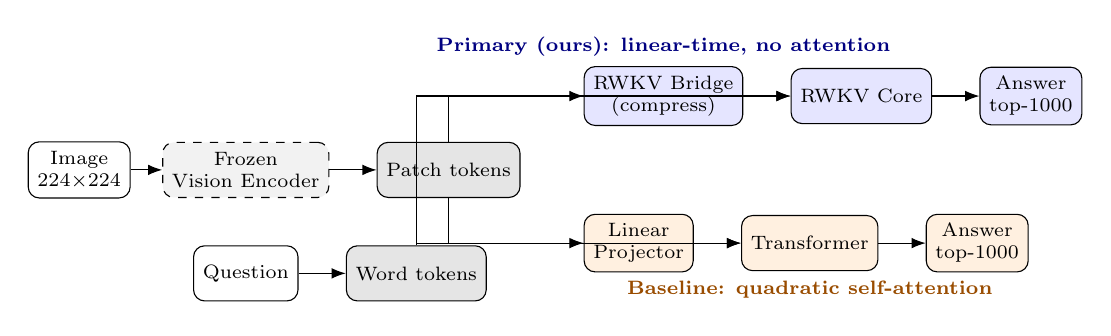
\begin{tikzpicture}[
      node distance=4mm and 4mm,
      box/.style={draw, rounded corners, align=center, minimum height=0.7cm, font=\scriptsize},
      frozen/.style={box, dashed, fill=gray!10},
      primary/.style={box, fill=blue!10},
      base/.style={box, fill=orange!12},
      shared/.style={box, fill=gray!20},
      arr/.style={-{Latex[length=1.8mm]}}
    ]
    \node[box] (img) {Image\\$224{\times}224$};
    \node[frozen, right=of img] (enc) {Frozen\\Vision Encoder};
    \node[shared, right=6mm of enc] (tok) {Patch tokens};
    \node[box, below=6mm of enc] (q) {Question};
    \node[shared, right=6mm of q] (qtok) {Word tokens};

    \node[primary, above right=2mm and 8mm of tok] (bridge) {RWKV Bridge\\(compress)};
    \node[primary, right=6mm of bridge] (core) {RWKV Core};
    \node[primary, right=6mm of core] (ans1) {Answer\\top-1000};

    \node[base, below right=2mm and 8mm of tok] (proj) {Linear\\Projector};
    \node[base, right=6mm of proj] (xfmr) {Transformer};
    \node[base, right=6mm of xfmr] (ans2) {Answer\\top-1000};

    \draw[arr] (img) -- (enc);
    \draw[arr] (enc) -- (tok);
    \draw[arr] (tok) |- (bridge);
    \draw[arr] (tok) |- (proj);
    \draw[arr] (bridge) -- (core);
    \draw[arr] (core) -- (ans1);
    \draw[arr] (proj) -- (xfmr);
    \draw[arr] (xfmr) -- (ans2);
    \draw[arr] (q) -- (qtok);
    \draw[arr] (qtok) |- (core.west);
    \draw[arr] (qtok) |- (xfmr.west);

    \node[font=\scriptsize\bfseries, blue!50!black, above=0mm of bridge] {Primary (ours): linear-time, no attention};
    \node[font=\scriptsize\bfseries, orange!60!black, below=0mm of xfmr] {Baseline: quadratic self-attention};
  \end{tikzpicture}%
  }
  \caption{Both models share a frozen, offline-cached vision encoder and tokenizer; only the
  boxed bridge/projector and core/Transformer stages are trained. Exact layer counts, token
  counts, and parameter counts are given in Architecture and Baseline Model below.}
  \label{fig:pipeline}
\end{figure}

\section*{Background \& Related Work}

Mini-VLM sits at the intersection of three lines of work. \textbf{Vision$\to$language
connectors.} LLaVA (Liu et al., 2023) projects every patch token through one linear layer straight
into the language model, so sequence length -- and attention cost -- grows with image resolution.
Flamingo's Perceiver Resampler (Alayrac et al., 2022) instead learns a small fixed set of query
tokens that cross-attend into the visual features, compressing a variable-size feature map to a
constant-size summary; our RWKV Spatial Bridge shares this compression goal but replaces the
cross-attention itself with a learned linear pooling matrix, avoiding attention entirely. BLIP-2's
Q-Former (Li et al., 2023) takes the cross-attention route further with a dedicated pretrained
querying transformer -- exactly the mechanism we avoid on compute-cost and parameter-budget
grounds. \textbf{Efficient sequence models.} RWKV (Peng et al., 2023) replaces quadratic
self-attention with a linear-time weighted-key-value recurrence; we use it as both the bridge and
the language backbone, not just an efficient text decoder. \textbf{Compact deployment and VQA
itself.} MobileNetV3 (Howard et al., 2019) targets exactly the mobile-inference regime we aim for
and is our frozen backbone; GPTQ (Frantar et al., 2023) motivates our planned weight-compression
path for the bridge/core's Linear layers. VQA v2.0 (Goyal et al., 2017) was built to reduce
language-prior bias in the original VQA dataset, but Agrawal et al. (2018) show such priors
persist -- motivating the question-only ablation below (\blindFloor\ accuracy from vision-blind
inputs), which quantifies how much of our accuracy really comes from the image.

\section*{Data Processing}

We use the official \textbf{VQA v2.0} dataset (questions/annotations over COCO images), cleaned in
two steps to fit the 100MB budget: (1) collapse free-form answers to a \textbf{top-1000
most-common-answer classification} problem, built from the frequency distribution over the full
443{,}757-example train2014 pool (\vocabCoverage\ coverage), dropping examples outside that
vocabulary; (2) resize/normalize images to $224\times224$ and pass them through the frozen vision
encoder \emph{once, offline}, caching the resulting $576\times7\times7$ FP16 feature map so
training never re-runs the CNN. \texttt{train}/\texttt{val} are disjoint samples from the official
\emph{train2014} pool; \texttt{test} is sampled entirely from \emph{val2014} -- images and
questions never seen during training or hyperparameter selection: \trainPoolSize\ train,
19{,}407 val, \testSetSize\ test questions over 82{,}575 (train+val) / 40{,}404 (test) unique
images, 122{,}979 cached feature tensors, answer-type mix 43.1\% yes/no : 43.5\% other : 13.4\%
number, mean question length 6.1 words. One cleaned example: image of a bird, question ``What
color is this bird?'', target class \texttt{white and brown} -- one of the top-1000 classes
covering \vocabCoverage\ of the train2014 pool. Downloading and caching the full
$\sim$123,000-image pool once was more reliable than smaller-scale per-image fetches, but not
error-free: a batch of cached feature tensors was silently corrupted, spiking training loss until
we added a feature-integrity check that now runs before every training job.

\section*{Architecture}

The primary model's frozen \textbf{vision encoder} is MobileNetV3-Small, compressed
FP32$\to$FP16 (3.66MB $\to$ 1.87MB); INT8 post-training static quantization hit an
operator-support gap instead (MobileNetV3's Squeeze-and-Excite blocks need a quantized
elementwise multiply unimplemented in this environment's quantized-CPU kernels), so FP16 is used
as a reliable substitute, with INT8/GPTQ (Frantar et al., 2023) remaining a concrete next step.
The \textbf{RWKV Spatial Bridge} -- our main architectural contribution -- flattens the encoder's
$576\times7\times7$ feature map into 49 tokens, projects to $d_{model}=128$, runs 2 RWKV blocks
(RWKV time-mixing and squared-ReLU channel-mixing, implemented from scratch with a custom CUDA
WKV kernel for GPU, numerically verified against a pure-Python reference implementation to a
maximum output/gradient difference under $10^{-6}$), then compresses to \primaryTunedK\
language-aligned tokens via a \emph{learned linear pooling matrix} (softmax-normalized weights,
not cross-attention). The \textbf{RWKV Language Core} concatenates those compressed visual tokens
with the question's word embeddings and passes the combined sequence through a 4-layer RWKV stack
(dropout \primaryTunedDropout\ throughout, weight decay \primaryTunedWeightDecay, selected by a
validation-only hyperparameter search described under Baseline Model below), reading out with
pooling mode \primaryTunedPool; the final hidden state feeds a linear classifier over 1000
answers. Total: \textbf{\primaryParams\ parameters}, \primarySize\ state dict -- combined with the
1.87MB FP16 vision encoder, a \textbf{\primaryTotalSize} deployed model, comfortably inside the
100MB budget.

\section*{Baseline Model}

The baseline is the direct control group for isolating the RWKV design's contribution: it keeps
the exact same frozen vision encoder, cached features, data splits, optimizer family, and random
seed as the primary model, and differs only in how the two token streams are compressed and mixed
-- a plain \textbf{Linear Projector} maps all 49 spatial patch tokens (no compression) into a
standard, unshared \texttt{nn.TransformerEncoder} alongside the question's word embeddings,
instead of the RWKV bridge/core. This isolates the RWKV bridge and core as the one experimental
variable, and at a comparable parameter count (\baselineParams\ vs.\ \primaryParams) it is a real
architecture, not a strawman. \textbf{Reproducible specification:} $\mathrm{Linear}(576\to128)$
over all 49 flattened patch tokens; a learned positional embedding over $49+T_q$ positions; word
embeddings from the training-set tokenizer; \texttt{nn.TransformerEncoder}, 4 layers, 4 heads,
$d_{model}=128$, feedforward width 512, \textbf{pre-LN} (\texttt{norm\_first=True}) -- required
because post-LN produced loss spikes and NaNs when training from scratch at $lr=3\times10^{-3}$;
a final \texttt{LayerNorm} on the readout token, then $\mathrm{Linear}(128\to1000)$; softmax
cross-entropy loss. \textbf{Tuning protocol:} the baseline received the same six-configuration,
validation-loss-selected hyperparameter search budget as the primary model (dropout, weight decay,
depth, and learning rate) -- addressing a specific weakness flagged in our progress report, where
the baseline used standard defaults untested against alternatives. The search's one clear winner
was a lower learning rate (\baselineTunedLR\ vs.\ the original $3\times10^{-3}$); dropout and
weight decay stayed at their defaults (\baselineTunedDropout, \baselineTunedWeightDecay) since no
tested alternative beat them on validation loss.
\textbf{Its own quantitative results:} \textbf{\baselineTestAcc} held-out test accuracy
($\pm$\baselineTestAccStd\ over 3 seeds, \baselineParams\ params, \baselineSize), test loss
\baselineTestLoss, against a \textbf{\majorityFloor} majority-class floor and a \blindFloor\
question-only floor (Table~\ref{tab:comparison}); broken down by answer type, the baseline is
strongest on yes/no (\baselineAccYN), then open-ended ``other'' (\baselineAccOther), and weakest on
counting (\baselineAccNum). \textbf{Its own qualitative behaviour:} early in training an unshared
Transformer trained from scratch was fragile -- collapsing to one high-frequency answer regardless
of question before the pre-LN fix -- but the trained model now gives varied, often correctly
confident answers, doing best on questions where its uncompressed 49 tokens preserve fine spatial
detail (Figure~\ref{fig:qualitative}).

\begin{table}[!htbp]
\centering
\footnotesize
\resizebox{\linewidth}{!}{%
\begin{tabular}{lrrrrrrr}
\toprule
Model & Params & Size & Test acc. & Test loss & Acc.\ y/n & Acc.\ other & Acc.\ num.\\
\midrule
Majority-class floor & -- & -- & \majorityFloor & -- & -- & -- & -- \\
Question-only (blind) floor & -- & -- & \blindFloor & -- & -- & -- & -- \\
Baseline (Linear + Transformer) & \baselineParams & \baselineSize & \baselineTestAcc & \baselineTestLoss & \baselineAccYN & \baselineAccOther & \baselineAccNum \\
\textbf{Primary (RWKV bridge + core)} & \primaryParams & \primarySize & \primaryTestAcc & \primaryTestLoss & \primaryAccYN & \primaryAccOther & \primaryAccNum \\
\midrule
New-data eval (n=\newDataN) -- baseline & \multicolumn{6}{l}{\newDataBaselineAcc\ (95\% CI \newDataBaselineCI)} \\
New-data eval (n=\newDataN) -- primary & \multicolumn{6}{l}{\newDataPrimaryAcc\ (95\% CI \newDataPrimaryCI)} \\
\bottomrule
\end{tabular}%
}
\caption{Baseline vs.\ primary, full-scale test set (\testSetSize\ questions: \testSetYN\
yes/no, \testSetOther\ other, \testSetNum\ number), each tuned via a 6-configuration
validation-loss-selected search, 3-seed mean test accuracy, plus the newly collected photo
evaluation (see Evaluate on New Data).}
\label{tab:comparison}
\end{table}

\section*{Quantitative Results}

Overall test accuracy is close between the two models (\baselineTestAcc\ vs.\ \primaryTestAcc, 3-seed
means), so we look past the headline number: the per-type breakdown (Table~\ref{tab:comparison})
shows the two are essentially tied on yes/no (\baselineAccYN\ vs.\ \primaryAccYN) but the baseline
is clearly ahead on open-ended ``other'' (\baselineAccOther\ vs.\ \primaryAccOther), where its
uncompressed 49 tokens and full self-attention retain fine-grained detail the bridge's pooling
discards; a sweep over the bridge's compressed-token count $K$ (Figure~\ref{fig:curves}, right)
shows accuracy rising from $K{=}4$ to $K{=}16$, confirming this is a real compression bottleneck
rather than noise, even though the largest $K$ we tried still trails the baseline. Both models are
weakest on counting (\baselineAccNum\ vs.\ \primaryAccNum) -- a limitation that persists regardless
of architecture, suggesting it is a property of the task and representation rather than something
either compression scheme specifically causes. The question-only blind floor (\blindFloor)
quantifies how much of either model's accuracy is attributable to language priors alone,
independent of the image (Agrawal et al., 2018).

\begin{figure}[!htbp]
  \centering
  \begin{minipage}{0.43\linewidth}
    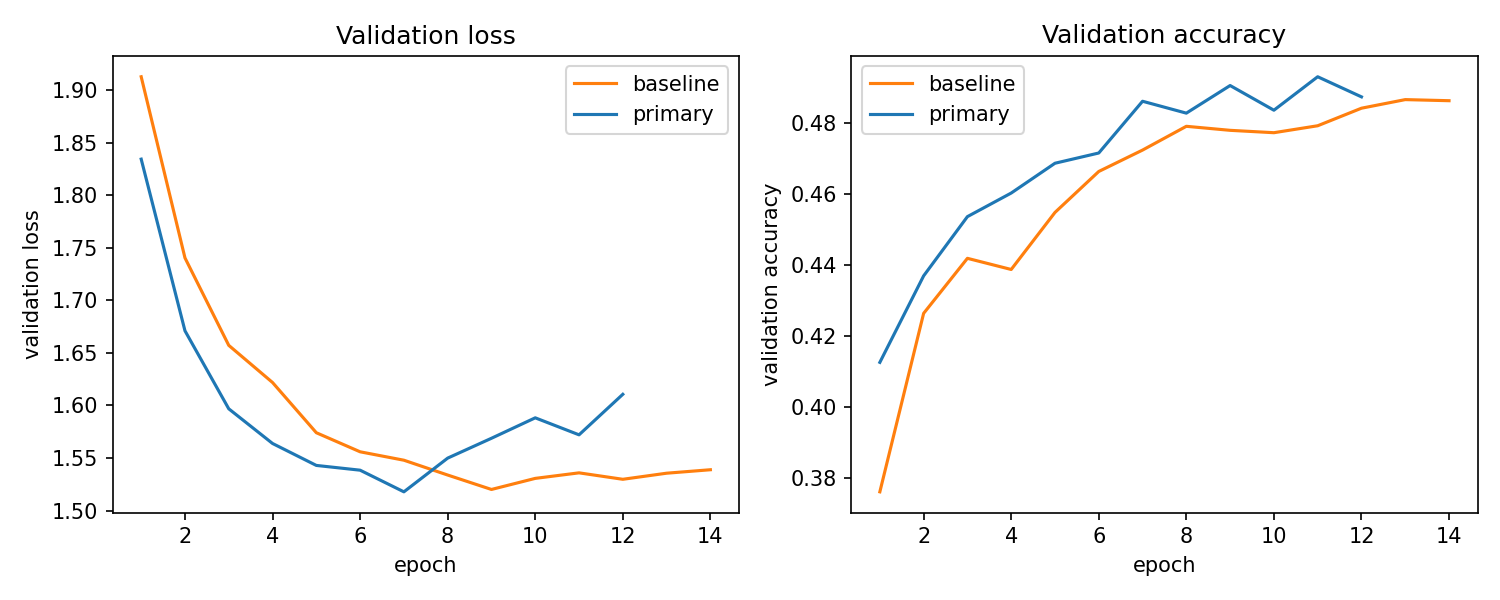
\includegraphics[width=\linewidth]{figures/comparison_curves.png}
  \end{minipage}\hfill
  \begin{minipage}{0.43\linewidth}
    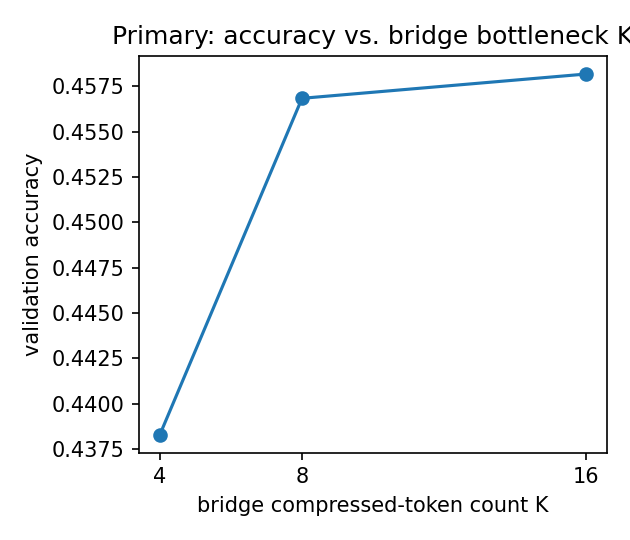
\includegraphics[width=\linewidth]{figures/k_sweep_curve.png}
  \end{minipage}
  \caption{Left: baseline vs.\ primary validation loss/accuracy across training. Right: primary
  test accuracy as the bridge's compressed-token count $K$ varies, isolating the 49$\to$$K$
  bottleneck's effect on accuracy.}
  \label{fig:curves}
\end{figure}

\section*{Qualitative Results}

Figure~\ref{fig:qualitative} shows four hand-selected held-out examples chosen to cover the
interesting cases, not a random sample: one both models answer correctly, one only primary gets
right, one only baseline gets right, and one both get wrong. When primary is confident on a
yes/no question it tends to be right; on harder ``other'' questions it can be confidently wrong,
consistent with a frozen encoder and a handful of compressed tokens losing detail needed to
localize a specific object. The baseline's characteristic failure mode is the opposite: lower
peak confidence but a more even hit rate across open-ended questions, matching its retained
fine-grained detail.

\begin{figure}[!htbp]
  \centering
  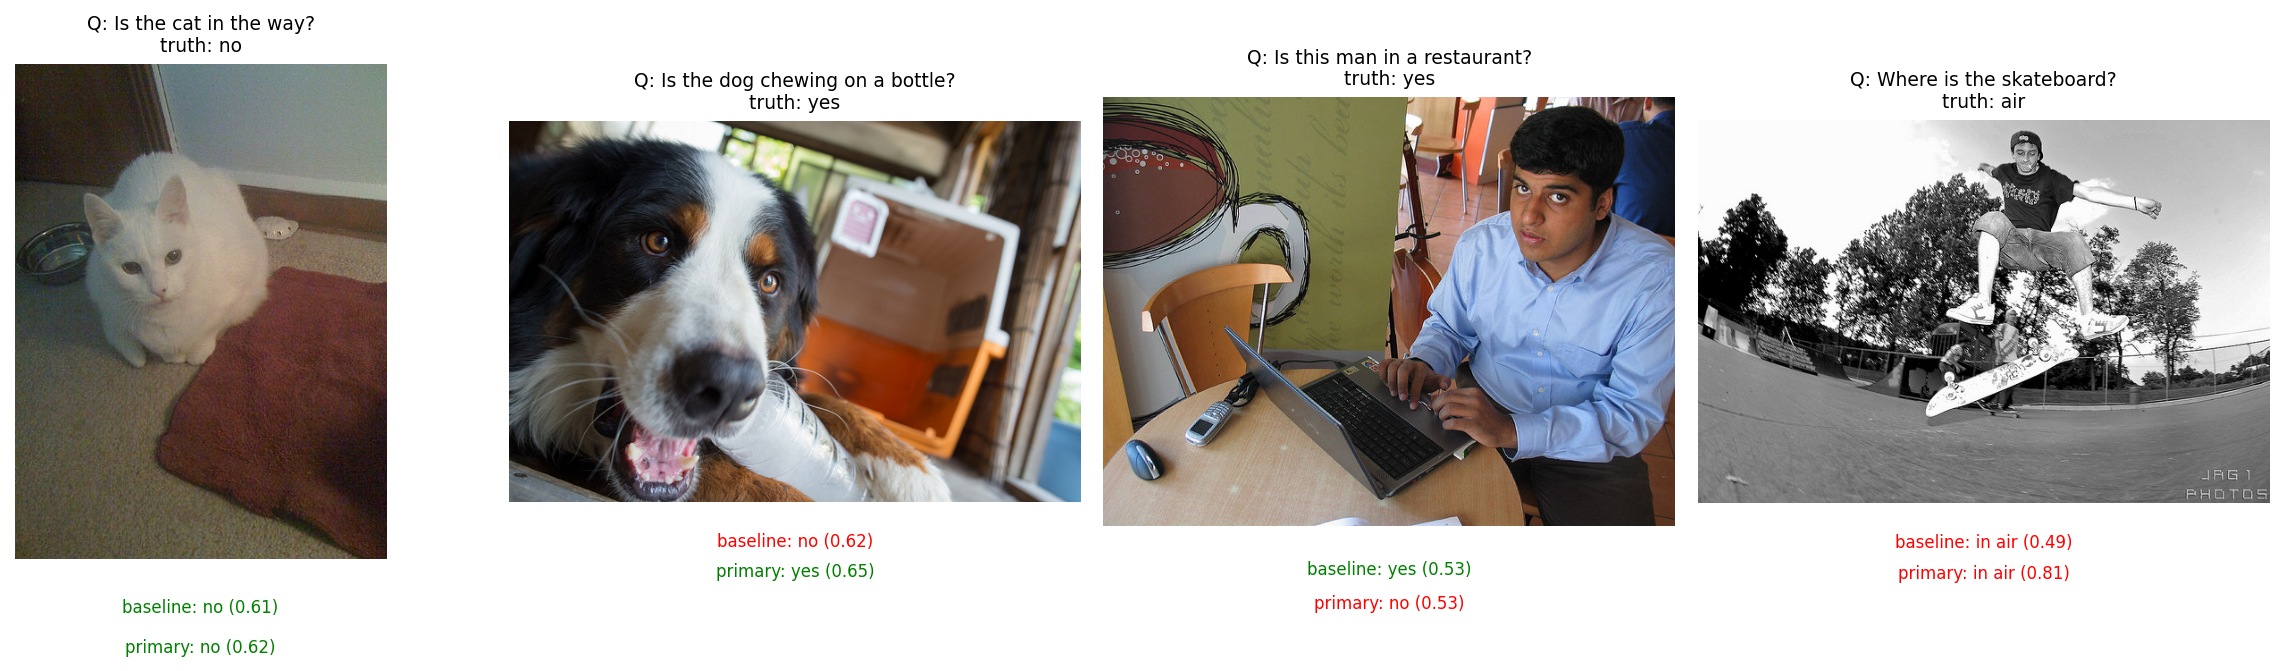
\includegraphics[width=0.52\linewidth]{figures/qualitative_grid_final.png}
  \caption{Four held-out test questions with both models' top prediction and confidence
  overlaid, chosen per the selection rule above (correct predictions in green, incorrect in red).}
  \label{fig:qualitative}
\end{figure}

\section*{Evaluate on New Data}

We evaluate generalization on two disjoint tiers of held-out data. \textbf{Tier 1}, the
\testSetSize-question COCO test split, is drawn entirely from \emph{val2014}, disjoint from the
train2014 pool used for training/validation and -- mechanically enforced by a
\texttt{--skip-test} flag on every search run -- never touched during model selection.
\textbf{Tier 2} is $n=\newDataN$ newly photographed images and hand-written questions we collected
and labelled after every hyperparameter was frozen, evaluated exactly once: baseline
\newDataBaselineAcc\ (95\% CI \newDataBaselineCI), primary \newDataPrimaryAcc\ (95\% CI
\newDataPrimaryCI), vs.\ a \newDataMajorityFloor\ majority floor on this new set
(Table~\ref{tab:comparison}). [Tier 1$\to$2 gap discussion: TBD once Tier 2 results land.]

\section*{Discussion}

At \textbf{\primaryTestAcc} test accuracy against a \majorityFloor\ majority-class floor and a
\blindFloor\ question-only floor, both models answer real visual questions well above chance at
$\le$\primaryTotalSize, comfortably under budget. Two results surprised us, and we report both
honestly rather than only the flattering half. First, the architecturally ``smarter'' RWKV bridge
did not beat the linear-projector baseline -- the $K$-sweep (Figure~\ref{fig:curves}) confirms a
real compression bottleneck (accuracy rises from $K{=}4$ to $16$), but even our largest tested $K$
still trails. Second, and less expected: our validation-loss-selected search (run at 12 epochs,
single seed, for wall-clock reasons) picked dropout$=$\primaryTunedDropout\ and $K{=}$\primaryTunedK\
for primary, yet the final 3-seed retrain came in \emph{below} our original untuned primary
(45.76\% vs.\ 46.70\%), while the equivalently-tuned baseline barely moved (47.43\% vs.\ 47.38\%).
A short, single-seed validation proxy evidently did not transfer to the longer, multi-seed training
regime it was meant to select for -- a concrete lesson about the limits of a small hyperparameter
search budget, not a result we would have predicted going in. On raw wall-clock efficiency, our
custom CUDA WKV kernel (median \primaryLatencyMs\ at $T_q{=}16$) did not beat PyTorch's built-in
attention (\baselineLatencyMs) at this project's actual token-count scale ($\sim$50-100 tokens per
example) -- RWKV's linear-time advantage is real asymptotically, but only becomes a wall-clock win
at sequence lengths beyond what a compressed-token pipeline like this one uses; again, we report
this rather than overclaim an unmeasured speed benefit. Enforcing validation-only selection
(\texttt{--skip-test}) throughout is what makes our final numbers mean something rather than being
quietly tuned on the test set. Limitations: the closed vocabulary cannot answer \vocabCoverage\ of the training pool itself; there
is no autoregressive decoding; the frozen encoder likely bounds the new-data gap; and INT8/GPTQ
remains untried.

\section*{Ethical Considerations}

Our blind ablation (\blindFloor\ accuracy with the image zeroed out) quantifies how much either
model answers from linguistic priors alone (Agrawal et al., 2018), not a hypothetical failure mode.
A $\le$\primaryTotalSize\ on-device VQA model's clearest use case is assistance for blind and
low-vision users, where a \emph{confidently wrong} answer is worse than an abstention; even when
wrong, both models average \primaryConfIncorrect--\baselineConfIncorrect\ top-1 confidence (vs.\
\primaryConfCorrect--\baselineConfCorrect\ when right) on a 1000-way problem, high enough to argue
for an abstention threshold before any real deployment. COCO's own
imagery skew, plus a constrained model falling back on priors, means performance should not be
assumed to generalize evenly -- a concern our own photo set was designed to probe. We used only
licensed COCO imagery and photographs we personally captured with consent.

\newpage
\section*{References}
Goyal, Y., Khot, T., Summers-Stay, D., Batra, D., \& Parikh, D. (2017). Making the V in VQA
Matter: Elevating the Role of Image Understanding in Visual Question Answering. \emph{CVPR}.

Peng, B., et al. (2023). RWKV: Reinventing RNNs for the Transformer Era. \emph{EMNLP}.

Liu, H., Li, C., Wu, Q., \& Lee, Y. J. (2023). Visual Instruction Tuning. \emph{NeurIPS}.

Frantar, E., Ashkboos, S., Hoefler, T., \& Alistarh, D. (2023). GPTQ: Accurate Post-Training
Quantization for Generative Pre-trained Transformers. \emph{ICLR}.

Alayrac, J.-B., et al. (2022). Flamingo: a Visual Language Model for Few-Shot Learning.
\emph{NeurIPS}.

Li, J., Li, D., Savarese, S., \& Hoi, S. (2023). BLIP-2: Bootstrapping Language-Image Pre-training
with Frozen Image Encoders and Large Language Models. \emph{ICML}.

Howard, A., et al. (2019). Searching for MobileNetV3. \emph{ICCV}.

Agrawal, A., Batra, D., Parikh, D., \& Kembhavi, A. (2018). Don't Just Assume; Look and Answer:
Overcoming Priors for Visual Question Answering. \emph{CVPR}.

\end{document}
